\documentclass{article}

\usepackage[letterpaper, portrait, margin=1in]{geometry}
\usepackage{siunitx}
\usepackage{tikz}
\usepackage{mathtools}
\usetikzlibrary{shapes,backgrounds}
\usepackage{graphicx}
\usepackage{amsmath}
\begin{document}

\title{Dyanmics Equations for Smartmouse 2018}
\author{Peter Mitrano}

\maketitle

Deriving the kinematic equations of a differential drive robot.

In micromouse, we consider the coordinate system where the robot begins in the bottom left hand corner facing North. Positive X is west, and positive Y is north. Z faces upward out of the maze. Theta of zero is facing west, along the positive X axis.

\textbf{TODO: Make all the code agree with this}.

\hfill

\begin{figure}[h]
  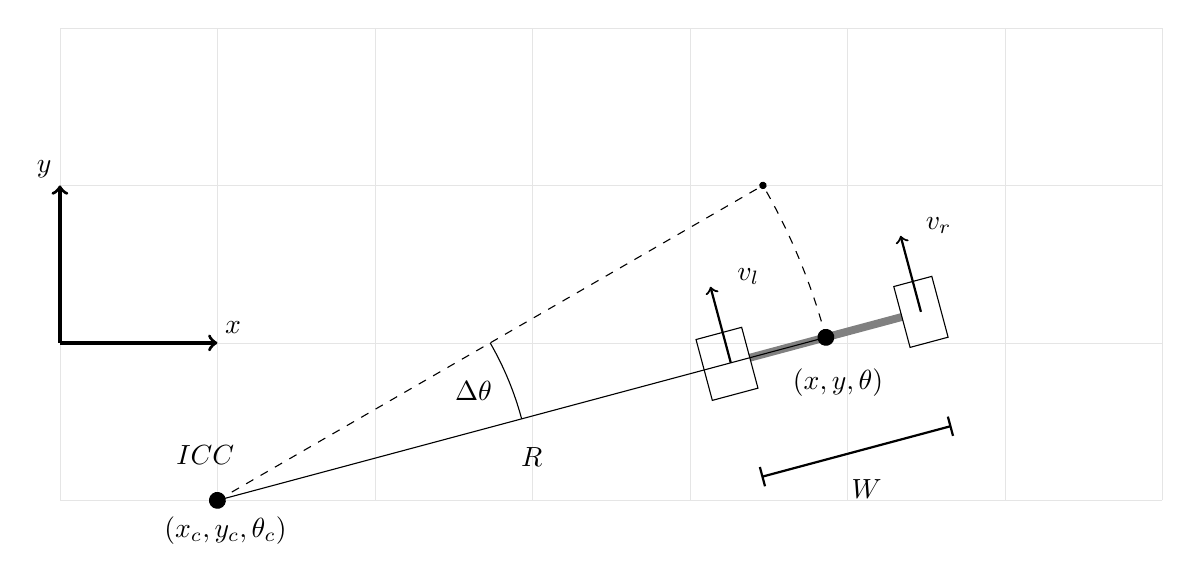
\begin{tikzpicture} [scale=2]
    % coordinate frame and grid%
    \definecolor{lg}{rgb}{0.9,0.9,0.9}
    \draw[step=1,lg,very thin] (-1,0) grid (6,3);
    \draw [very thick,->] (-1,1) -- (-1,2);
    \draw [very thick,->] (-1,1) -- (0,1);
    \draw (-1.1, 2.1) node {$y$};
    \draw (0.1, 1.1) node {$x$};

    % robot and stuff %
    \draw [line width=1mm, draw=gray,rotate around={15:(0,0)}]{(3.5,0)--(4.5, 0)};
    \draw [rotate around={15:(0,0)}] {(3.2,-0.2) rectangle (3.5, 0.2)};
    \draw [rotate around={15:(0,0)}] {(4.5,-0.2) rectangle (4.75, 0.2)};
    \draw [rotate around={15:(0,0)}] {(0,0) -- (4, 0)};
    \draw [dashed,rotate around={30:(0,0)}] {(0,0) -- (4, 0)};
    \draw [dashed,rotate around={15:(0,0)}] (4,0) arc (0:15:4);
    \draw [rotate around={15:(0,0)}] (2,0) arc (0:15:2);
    \draw [thick,->,rotate around={15:(0,0)}] (3.375,0) -- (3.375,0.5);
    \draw [thick,->,rotate around={15:(0,0)}] (4.625,0) -- (4.625,0.5);
    \draw [thick,|-|,rotate around={15:(0,0)}] (3.375,-0.75) -- (4.625,-0.75);
    \filldraw [rotate around={15:(0,0)}] {(0,0) circle (.05)};
    \filldraw [rotate around={15:(0,0)}] {(4,0) circle (.05)};
    \filldraw [rotate around={30:(0,0)}]{(4,0) circle (.02)};
    \draw [rotate around={15:(0,0)}] (1.75, 0.25) node {$\Delta\theta$};
    \draw [rotate around={15:(0,0)}] (3.625, 0.5) node {$v_l$};
    \draw [rotate around={15:(0,0)}] (4.875, 0.5) node {$v_r$};
    \draw [rotate around={15:(0,0)}] (2, -0.25) node {$R$};
    \draw [rotate around={15:(0,0)}] (4, -1) node {$W$};
    \draw [rotate around={15:(0,0)}] (4, -.3) node {$(x,y,\theta)$};
    \draw [rotate around={15:(0,0)}] (0, 0.3) node {$ICC$};
    \draw [rotate around={15:(0,0)}] (0, -.2) node {$(x_c,y_c,\theta_c)$};
  \end{tikzpicture}
  \centering
\end{figure}

At an instant in time we say that the robot is turning around some point $ICC$, the instanteous center. The radius $R$ about that point is what we want to solve for. We start with the knowedge that since the robot doesn't tear itself apart while driving, the rate $\omega$ at which both wheels (and the robot) move around $ICC$ is the same.
\begin{equation} \label{eq:1}
  \omega_l = \omega_r = \omega
\end{equation}
Let $R_l$ and $R_l$ be the radius to the right and left wheels.
\begin{equation} \label{eq:2}
  \omega = \frac{v_l}{R_l} = \frac{v_r}{R_r}
\end{equation}
We can then combine \ref{eq:1} and \ref{eq:2}
\begin{equation}
  \frac{v_l}{R_l} = \frac{v_r}{R_r}
\end{equation}
We can then substitute $R_l = R - \frac{W}{2}$ and $R_r = R + \frac{W}{2}$
\begin{equation}
  \frac{v_l}{R-\frac{W}{2}} = \frac{v_r}{R + \frac{W}{2}}
\end{equation}

Now do some algebra...
\begin{align*}
  \frac{v_l}{R-\frac{W}{2}} &= \frac{v_r}{R + \frac{W}{2}} \\[1em]
  \frac{R-\frac{W}{2}}{v_l} &= \frac{R + \frac{W}{2}}{v_r} \\[1em]
  \frac{R}{v_l}-\frac{W}{2v_l} &= \frac{R}{v_r} + \frac{W}{2v_r} \\[1em]
  \frac{R}{v_l}-\frac{R}{v_r} &= \frac{W}{2v_r}+\frac{W}{2v_l} \\[1em]
  \frac{2R(v_r-v_l)}{v_rv_l} &= \frac{W(v_l+v_r)}{v_rv_l} \\[1em]
  2R(v_r-v_l) &= W(v_l+v_r) \\[1em]
  R &= \frac{W(v_l+v_r)}{2(v_r-v_l)} \\[1em]
\end{align*}

We can use this result to get a cleaner equation for $\omega$, which right now requires diving by $R$. This is problematic because $R$ can be $0$.

\begin{align*}
  \omega &= \frac{v_l}{R-\frac{W}{2}}\\[1em]
         &= \frac{v_l}{\frac{W(v_l+v_r)}{2(v_r - v_l)}-\frac{W}{2}}\\[1em]
         &= \frac{v_l}{\frac{W(v_l+v_r)}{2(v_r - v_l)}-\frac{W(v_r - v_l)}{2(v_r - v_l)}}\\[1em]
         &= \frac{v_l}{\frac{W(v_l+v_r)-W(v_r - v_l)}{2(v_r - v_l)}}\\[1em]
         &= \frac{2v_l(v_r - v_l)}{W(v_l+v_r)-W(v_r - v_l)}\\[1em]
         &= \frac{2v_l(v_r - v_l)}{Wv_l+Wv_r-Wv_r+Wv_l}\\[1em]
         &= \frac{2v_l(v_r - v_l)}{2Wv_l}\\[1em]
         &= \frac{v_r - v_l}{W}\\[1em]
\end{align*}


\textbf{Next we need to figure out how to update our $x$, $y$, and $\theta$ given $R$.} \\

Before we can solve any of these, we need to figure out what $\Delta\theta$ is equal to. We will assume we are following this arc of constant radius for a given time step $\Delta t$. This is a good assumption if our time step is equal to our controller time step, during which presumably the speeds of the motors aren't changing, and so neither will our turning radius. If so, then $\Delta\theta = \omega\Delta t$, and we know
$$\omega=\frac{v_r - v_l}{W}$$
Lets just pick $v_l$, and put them together to get $\Delta\theta$.
$$\Delta\theta = \frac{v_r - v_l}{W}\Delta t$$

So what are our update equations? Theta is obvious: $\theta \leftarrow \theta+\Delta\theta$. The coordinates of $ICC = (x-R\sin{\theta}, y+R\cos{\theta})$. You can see this if you think that the vector to $ICC$ is 90 degrees offset from $\theta$ and do the trig. Let's assume in the situation diagramed above, $\theta=\ang{105}$, $R=4$, and $x=4.8, y=0$, so $ICC = (4.8-4\sin{(105)}, 0+4\cos{(105)}) \approx (1, -1)$. For another example, pretend the robot is right below the origin facing east at $(0,-1,0)$ and $R=1$. $ICC$ should be $(0,0)$ so let's check. $ICC = (0-1\sin{(0)}, -1+1\cos{(0)}) = (0, 0).$ Great, the math seems to check out. Now we just rotate the robot coordinates around the point $ICC$ by $\Delta\theta$, which we can do easily with a rotation matrix. Of course, we're not rotating around the origin, we're roating around $ICC$, so we first subtract out the coordinates of $ICC$ to get $(x_o, y_o) = (x- ICC_x, y-ICC_y)$. Recall that to rotate around the origin by $\Delta\theta$, we multiply our point $(x_o, y_o)$ as follows:
\begin{equation}
  \begin{bmatrix}
    \cos{\Delta\theta} & -\sin{\Delta\theta} \\
    \sin{\Delta\theta} & \cos{\Delta\theta} \\
  \end{bmatrix}
  \begin{bmatrix}
    x_o \\
    y_o \\
  \end{bmatrix}
  =
  \begin{bmatrix}
    x_{new} \\
    y_{new} \\
  \end{bmatrix}
\end{equation}
We then just add back the coordinates of $ICC$. Great! Now we know how to update all our coordinates. Let's summarize:

\begin{align}
 \theta &\leftarrow \theta + \Delta\theta \\
  x &\leftarrow \cos{(\Delta\theta)}(x-ICC_x)-\sin{(\Delta\theta)}(y-ICC_y) + ICC_x \\
  y &\leftarrow \sin{(\Delta\theta)}(x-ICC_x)+\cos{(\Delta\theta)}(y-ICC_y) + ICC_y \\
\shortintertext{where}
  ICC_x &= x-R\sin{\theta} \\
  ICC_y &= y+R\cos{\theta} \\
  \Delta\theta &= \frac{v_r-v_l}{W}\Delta t \\
  R &= \frac{W(v_l+v_r)}{2(v_r-v_l)}
\end{align}

We can expand and simplify the udpate equations for $x$.

\begin{align}
  x &\leftarrow \cos{(\frac{v_r-v_l}{W}\Delta t)}(x-x+R\sin{\theta})-\sin{(\frac{v_r-v_l}{W}\Delta t)}(y-y-R\cos{\theta}) + x-R\sin{\theta} \\
  x &\leftarrow \cos{(\frac{v_r-v_l}{W}\Delta t)}(R\sin{\theta})-\sin{(\frac{v_r-v_l}{W}\Delta t)}(-R\cos{\theta}) + x-R\sin{\theta} \\
  x &\leftarrow R\cos{(\frac{v_r-v_l}{W}\Delta t)}\sin{\theta}+R\sin{(\frac{v_r-v_l}{W}\Delta t)}\cos{\theta} + x-R\sin{\theta} \\
  x &\leftarrow x+R\cos{(\frac{v_r-v_l}{W}\Delta t)}\sin{\theta}+R\sin{(\frac{v_r-v_l}{W}\Delta t)}\cos{\theta}-R\sin{\theta} \\
  x &\leftarrow x+R\Big(\cos{(\frac{v_r-v_l}{W}\Delta t)}\sin{\theta}+\sin{(\frac{v_r-v_l}{W}\Delta t)}\cos{\theta}\Big)-R\sin{\theta} \\
  \shortintertext{let $\frac{v_r-v_l}{W}=a$, and $\theta=b$, we can use $\cos{a}\sin{b}+\sin{a}\cos{b}=\sin{(a+b)}$}
  x &\leftarrow x+R\Bigg(\sin{\Big(\frac{v_r-v_l}{W}\Delta t+\theta}\Big)\Bigg)-R\sin{\theta} \\
  x &\leftarrow x+R\Bigg(\sin{\Big(\frac{v_r-v_l}{W}\Delta t+\theta}\Big)-\sin{\theta}\Bigg) \\
\end{align}

We can apply the same process for $y$.

\begin{align}
  y &\leftarrow y-R\Bigg(\cos{\Big(\frac{v_r-v_l}{W}\Delta t+\theta\Big)}-\cos{\theta}\Bigg)
\end{align}

\textbf{Final Solution to the forward Kinematics:}
\begin{align}
 \theta &\leftarrow \theta + \frac{v_r-v_l}{W}\Delta t \\
  x &\leftarrow x+R\Bigg(\sin{\Big(\frac{v_r-v_l}{W}\Delta t+\theta\Big)}-\sin{\theta}\Bigg) \\
  y &\leftarrow y-R\Bigg(\cos{\Big(\frac{v_r-v_l}{W}\Delta t-\theta\Big)}-\cos{\theta}\Bigg)
\end{align}

However, there is also the case where the robot is going perfectly straight. This has to be handled seperately, because otherwise the equations above involve $R$, but $R=\infty$ if we're going straight. Luckily, the equations for moving straight are trivial:
\begin{align}
 \theta &\leftarrow \theta \\
  x &\leftarrow x + v\Delta t\cos(theta) \\
  y &\leftarrow y + v\Delta t\sin(theta) \\
\end{align}

Here, $v$ can be $v_l$, or $v_r$ since they should be the same. In code, a simple average is used to correct for any slight numerical inconsistencies. \\

We must also consider how to model the DC Motors. \\

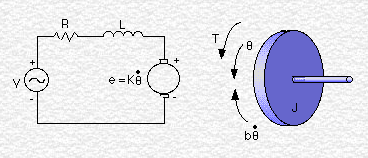
\includegraphics[scale=0.5]{./dc_motor_model.png}

The motor torque, $T$, is related to the armature current, $i$, by a constant factor $K$. The back emf, $e$, is related to the rotational velocity by the following equations:
$$T=Ki$$
$$e=K\dot{\theta}$$

From the figure above we can write the following equations based on Newton's law combined with Kirchhoff's law:
$$J\frac{d}{dt}\dot{\theta} + b\dot{\theta} = Ki$$
$$L\frac{d}{dt}i+Ri=V-K\dot{\theta}$$

In state-space form, the equations above can be expressed by choosing the rotating speed and electric current as the state variables and the voltage as an input. The output is chosen to be the rotating speed. The general linear state-space form is $\dot{X} = AX + BW$. We can get the two equations above in this form with some algebra.
\begin{align}
  J\frac{d}{dt}\dot{\theta} + b\dot{\theta} &= Ki \\
  \frac{d}{dt}\dot{\theta} + \frac{b\dot{\theta}}{J} &= \frac{Ki}{J} \\
  \frac{d}{dt}\dot{\theta} &= \frac{Ki}{J} - \frac{b\dot{\theta}}{J}
\end{align}

\begin{align}
  L\frac{d}{dt}i + Ri &= V - K\dot{\theta} \\
  \frac{d}{dt}i + \frac{Ri}{L} &= \frac{V}{L} - \frac{K\dot{\theta}}{L} \\
  \frac{d}{dt}i &= \frac{V}{L} - \frac{K\dot{\theta}}{L} - \frac{Ri}{L}
\end{align}

Next we combine these in a matrix.

\begin{align}
  \frac{d}{dt}\begin{bmatrix}\dot{\theta}\\i\\\end{bmatrix} &=
    \begin{bmatrix}
      \frac{-b}{J} & \frac{K}{J} \\
      \frac{-K}{L} & \frac{-R}{L} \\
    \end{bmatrix}
    \begin{bmatrix}
      \dot{\theta} \\
      i
    \end{bmatrix}
    +
    \begin{bmatrix}
      0 \\
      \frac{1}{L}
    \end{bmatrix}
    V
\end{align}

What this gives us is a nice matrix-y formula for the change in the current and angle of our motor over time. We can use this equation to simulate the behavior of the motor. If we assume the motor start at some initial $\dot{\theta}$, $i_0$ and $\dot{i}$, and we know all our motor constants ($K$, $R$, $L$, $b$, $J$) we can figure out the right hand side of the equation, and the result will be how much $i$ and $\dot{\theta}$ changes over some discrete time step. That is what we do in the smartmouse simulator server code.

\end{document}

